%++++++++++++++++++++++++++++++++++++++++
% Don't modify this section unless you know what you're doing!
\documentclass[letterpaper,12pt]{article}
\usepackage{tabularx} % extra features for tabular environment
\usepackage{setspace} 
\usepackage{amsmath}  % improve math presentation
\usepackage[portuguese]{babel}
\usepackage{graphicx} % takes care of graphic including machinery
\usepackage{titling}
\usepackage[margin=1in,letterpaper]{geometry} % decreases margins
\usepackage{cite} % takes care of citations
\usepackage[final]{hyperref} % adds hyper links inside the generated pdf file
\hypersetup{
	colorlinks=true,       % false: boxed links; true: colored links
	linkcolor=blue,        % color of internal links
	citecolor=blue,        % color of links to bibliography
	filecolor=magenta,     % color of file links
	urlcolor=blue         
}
%++++++++++++++++++++++++++++++++++++++++
\doublespacing
\title{PBL 1 - Monetária }
\author{ \name{João Pedro Miranda da Silva (Noite)}\\
\name{Paulo Francisco da Silva Júnior  (Manhã)}\\
\name{Pedro Henrique Aleluia de Moraes (Noite)}}

\begin{document}
\date{23 de Dezembro de 2022}
\maketitle
\begin{abstract}
Esse documento contém a resolução para o PBL 1 da cadeira de Monetária.
\end{abstract}

\section{Introdução}
De acordo com a teoria econômica a demanda agregada por ativos financeiros é negativamente correlacionada ao risco, ou seja, quanto maior o risco, menor a demanda por esse ativo. Nesse sentido, é importante separar o risco em duas categorias: Risco Agregado e Risco Idiossincrático. Para a análise desse caso, o tipo de risco que mais nos interessa é o agregado. Nesse sentido, o também chamado risco de mercado é o risco comum a todos os ativos negociados no mercado, estando relacionado a conjuntura econômica como um todo, sendo afetado por diversos fatores, tanto domésticos como internacionais. Com isso, é possível concluir que as escolhas dos indivíduos quanto aos ativos que serão adquiridos são altamente influenciadas pela conjuntura econômica global.

\section{Problema 1}
\paragraph{Elabore uma figura com as taxas de juros acumuladas (nominal e real) durante
os respectivos períodos de investimento de Maria e de Enzo entre janeiro de 2016 e novembro
de 2022. Baseado nessa figura, discuta sobre as diferentes reações das demandas individuais
por ativos financeiros de Enzo e Maria frente às mudanças dos riscos e das incertezas no início
da pandemia dado às informações disponíveis.}
\subsection{Resolução 1}

\begin{figure}[!tbh]
    \centering
    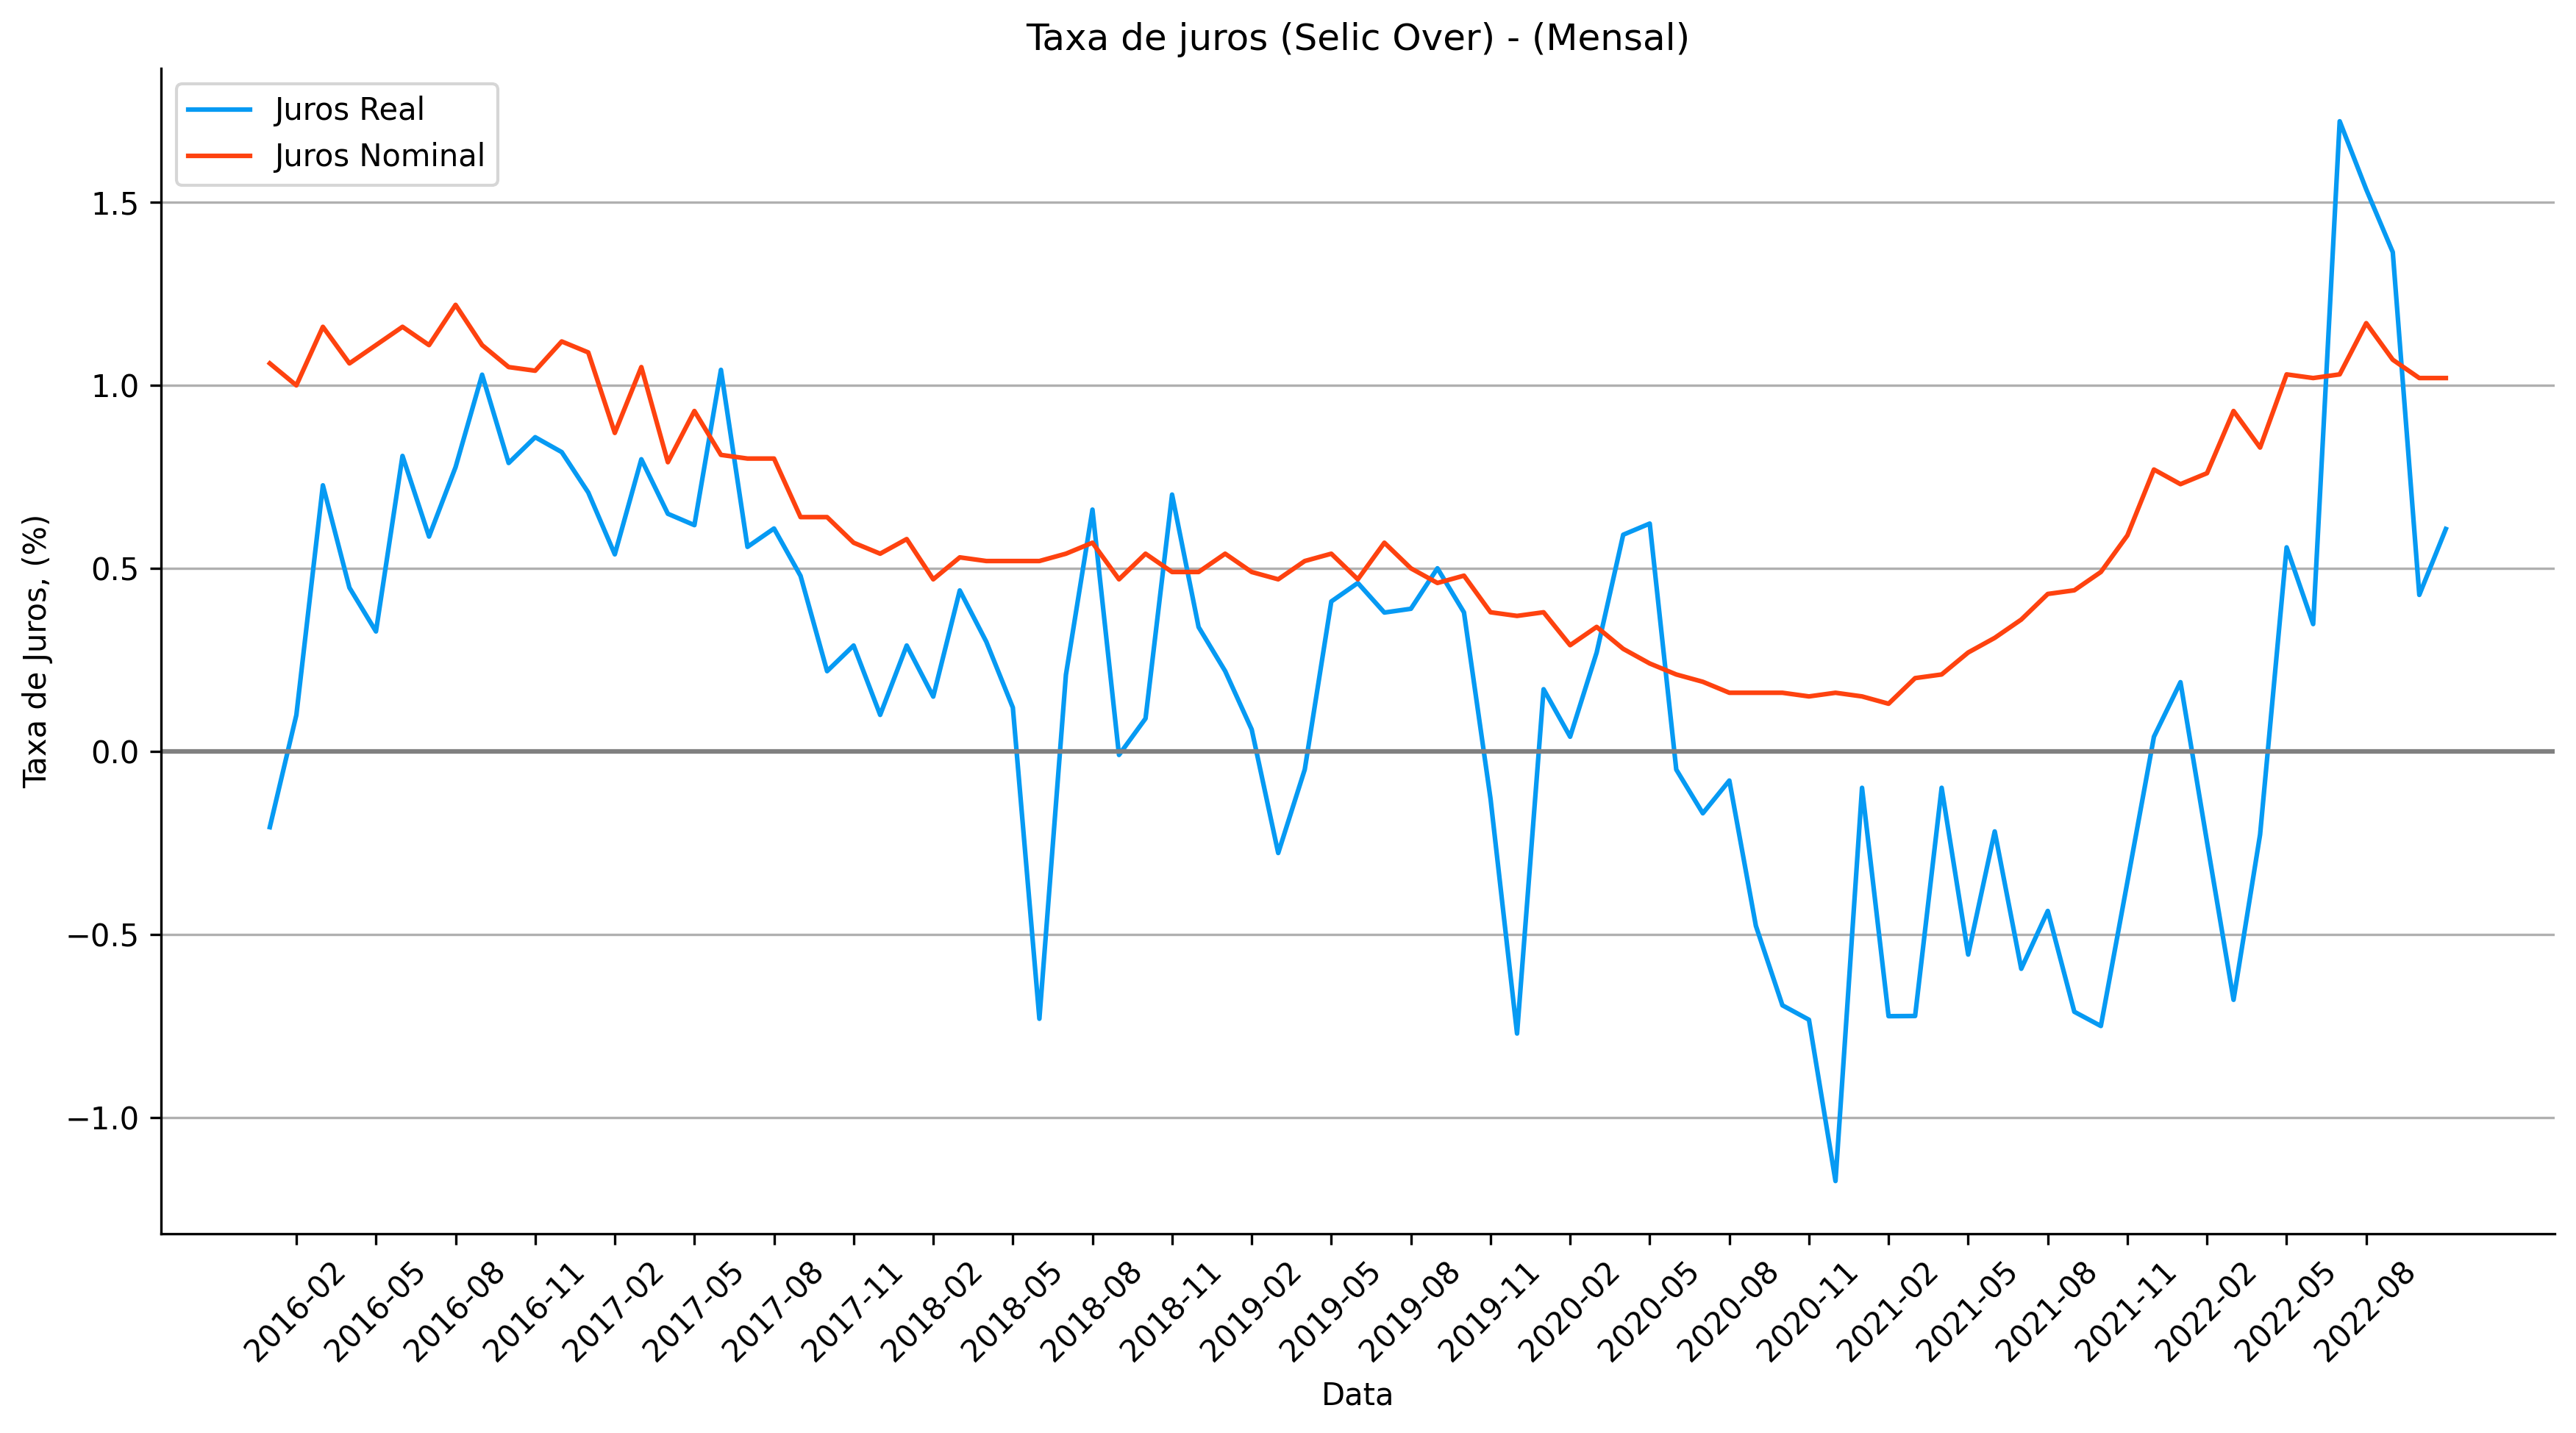
\includegraphics[width=\textwidth]{taxas.png}
    \caption{Taxa de juros Nominal e Real (Selic Over - Mensal, 2016-2022)}
    \label{fig:a}
\end{figure}

\begin{figure}[!tbh]
    \centering
    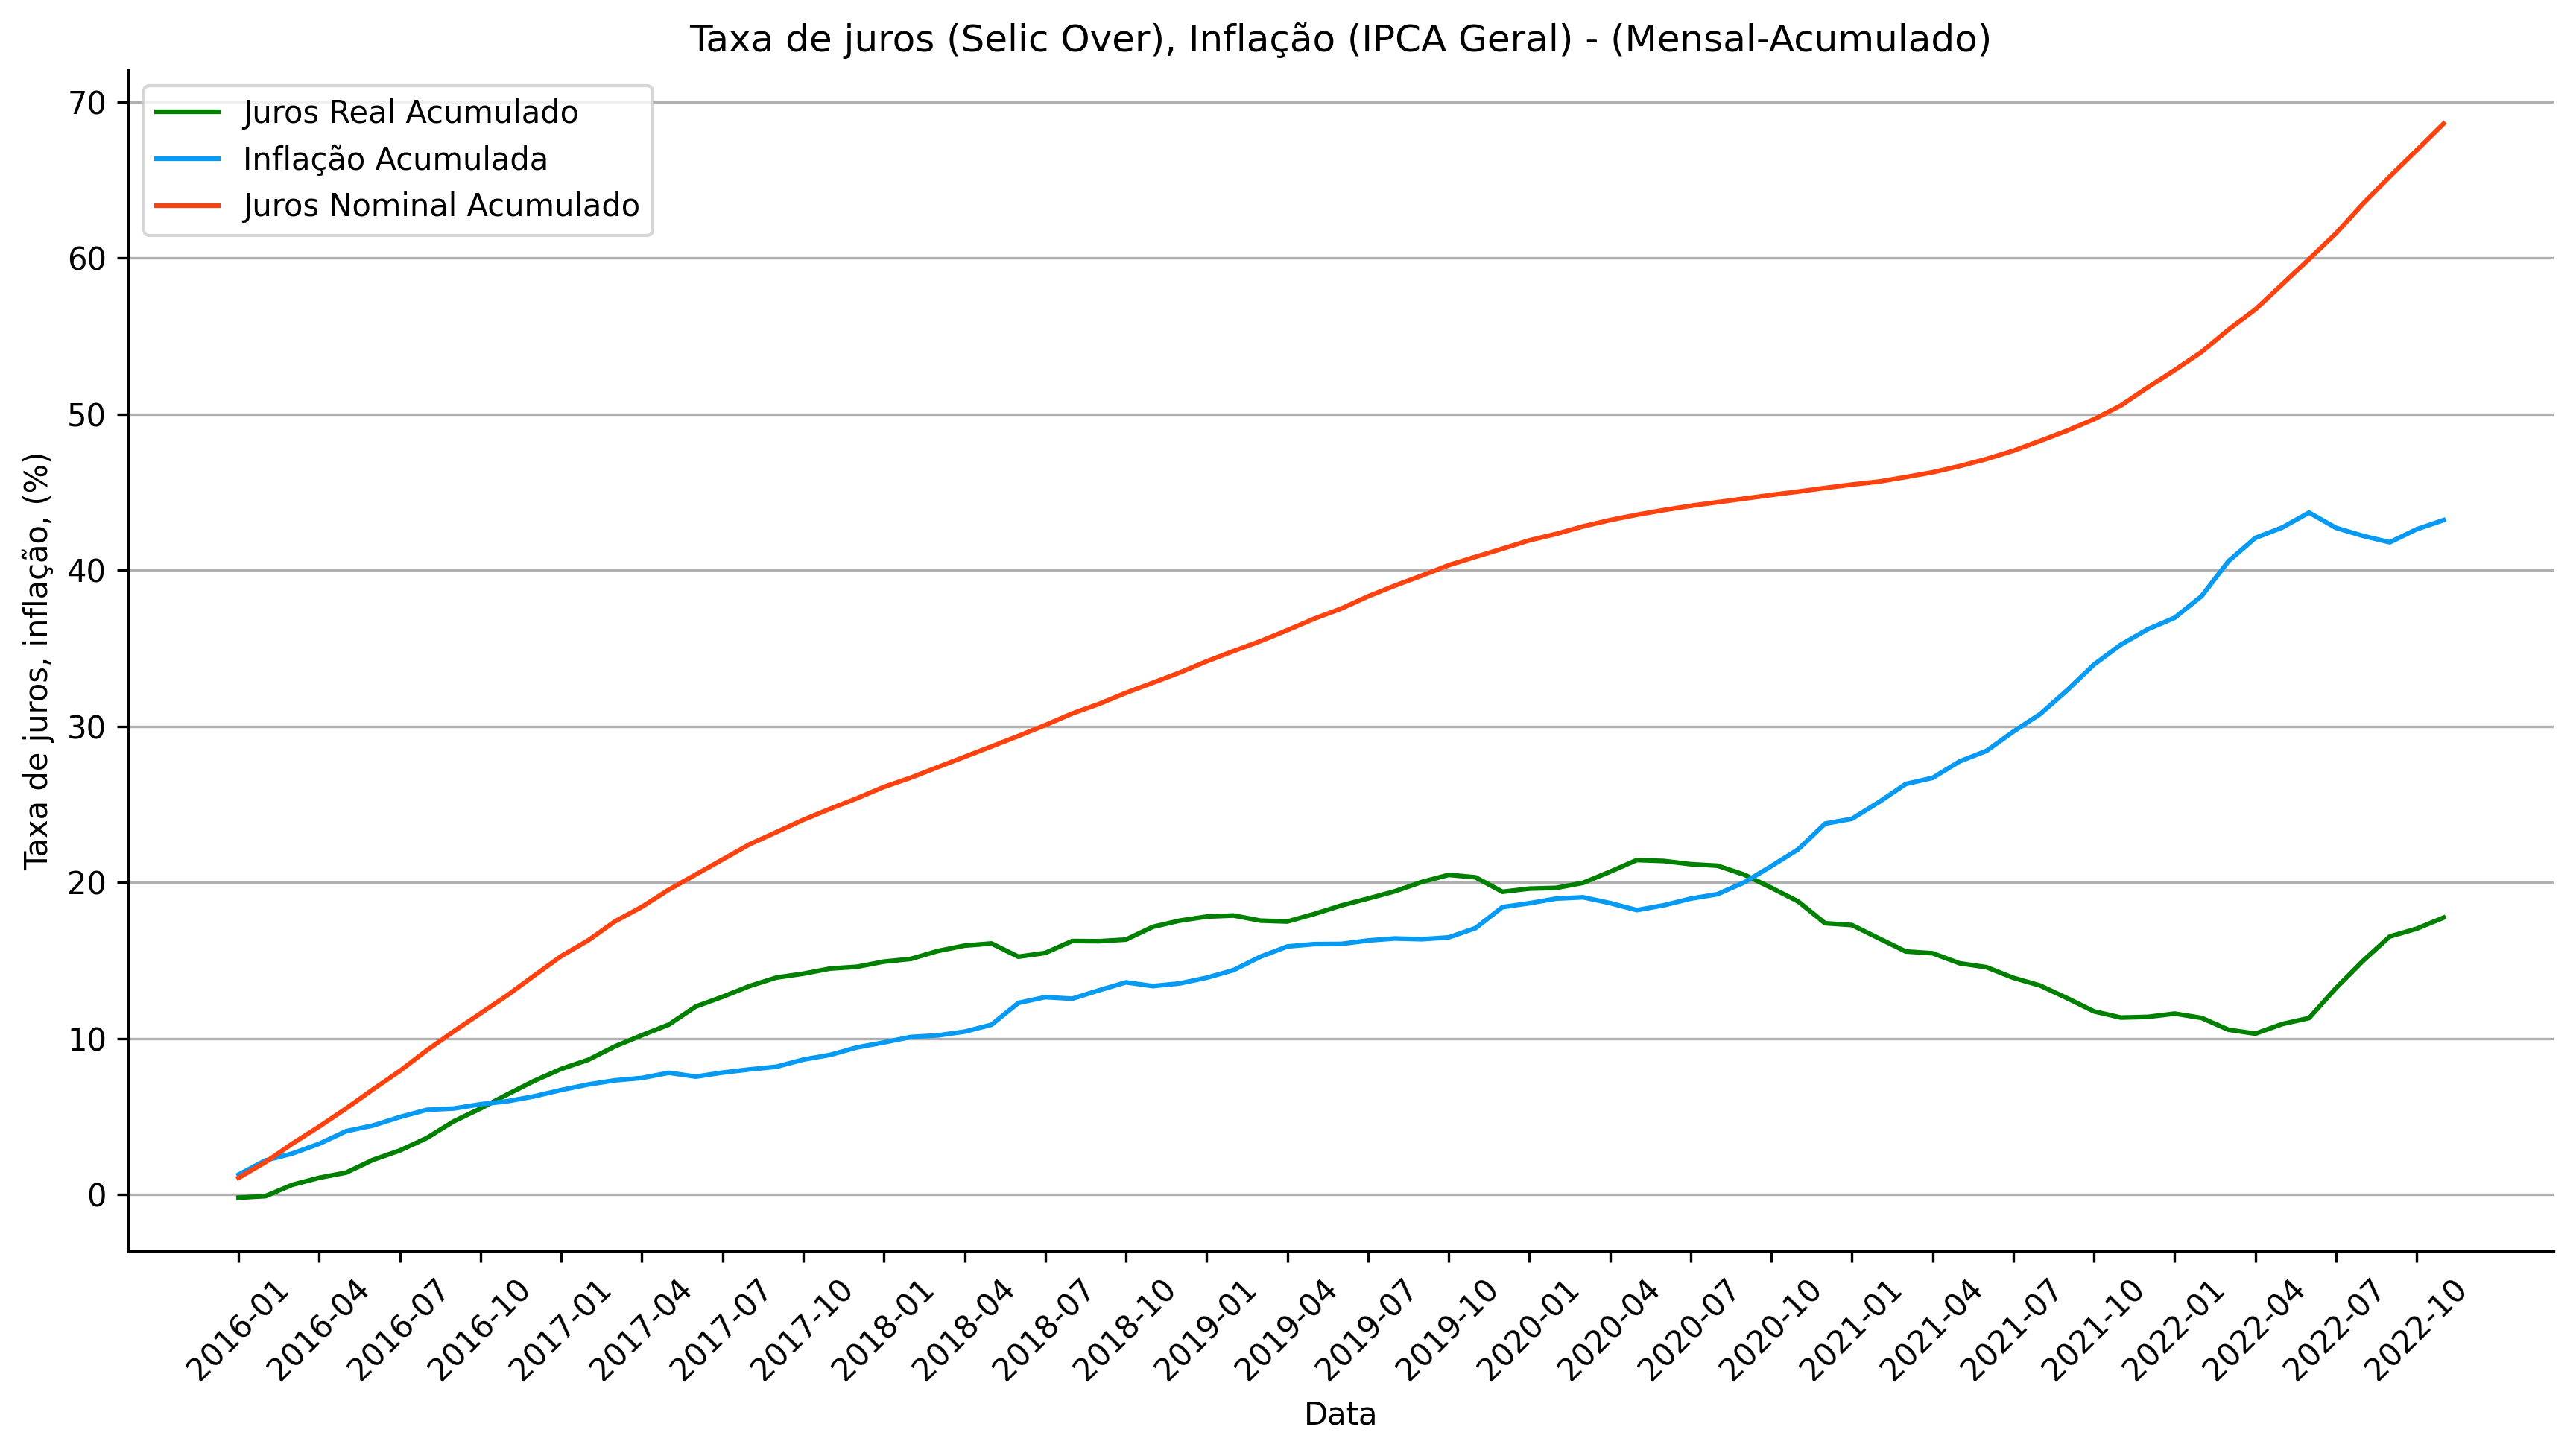
\includegraphics[width=\textwidth]{taxasAcumuladas.png}
    \caption{Taxa de juros Nominal e Real (Selic Over), Inflação (ICPA Geral) - Mensal}
    \label{fig:a}
\end{figure}
 \newpage
 
Com a chegada da covid-19 e suas consequências para economia global houve um aumento da incerteza mundial e do risco agregado. Nos gráficos podemos verificar que a partir do primeiro trimestre de 2020 a taxa de juros real acumulada entrou em tendência de queda fazendo com que o rendimento do ativo diminuísse, retraindo a demanda por este ativo. Enzo, por ter maior grau de aversão ao risco, comparado a Maria, chegou a conclusão de que preferiria liquidar sua posição frente à instabilidade global.


\section{Problema 2}

\paragraph{Em dezembro de 2022, Enzo e Maria estão reavaliando se mantém ou não
o produto de investimento dado às informações disponíveis. Frente ao cenário macro global,
quais seriam os motivos pelos quais Enzo ou Maria resgatariam o investimento? Quais seriam
os motivos pelos quais Enzo ou Maria manteriam o investimento?}
\subsection{Resolução 2}

A análise feita pelo Itaú mostra que o risco de recessão mundial caiu, sendo a previsão de crescimento PIB para 2023 de 2,3\%, e que a inflação que estava assolando a economia global desde 2020 está entrando em um processo de desaceleração, o que permitirá uma flexibilização do aperto monetário praticado pelos bancos centrais ao redor do mundo.

Porém, na América Latina, o cenário é um pouco mais incerto. No Brasil, por exemplo, existe uma grande preocupação no que diz respeito às políticas fiscais que serão adotas para os próximos anos. Gastos acima do teto e incertezas quanto a composição dos ministérios estão entre as preocupações dos investidores. Vale também ressaltar que, a projeção de crescimento para o Brasil em 2022 e 2023 foi elevada em meio à retomada das atividades econômicas

Com todas essas informações, podemos fazer uma análise mais precisa do problema 2. Nesse sentido, como foi supracitado, é pouco provável que ocorra cortes na taxa de juros básica da economia brasileira, fazendo com que o rendimento desse investimento se mantenha elevado por um período maior de tempo e, dessa forma, incentivando àqueles que têm os títulos a manterem. Por outro lado, com a redução da incerteza em outros países e com o aumento das internas - relacionadas às políticas públicas que podem ser adotadas, como, por exemplo, o furo no teto de gastos e grandes incentivos fiscais - Enzo e Maria podem trocar esse ativo doméstico por um estrangeiro, fugindo, assim, das incertezas e riscos domésticos.
\end{document}
